% !TeX spellcheck = ru_RU
% !TEX root=../main.tex

\begin{lecture}[Седьмая]
	\begin{lecSection}[Типы взаимодействий]
	\begin{flushleft}	
		\begin{itemize}
			\item Кулоновское $\propto $\Large$\frac{1}{\varepsilon r}$ \normalsize	
			\item Ион-ионное $\propto $\Large$\frac{1}{\varepsilon r^2}$ \normalsize
			\item Диполь-дипольное $\propto$\Large$\frac{1}{\varepsilon r^3}$\normalsize
			\item Ион-нейтральная частица $\propto$\Large$\frac{1}{\varepsilon^2 r^4}$\normalsize
			\item Нейтрал - нейтрал (В-д-В)(Дисперсное взаимодействие) $\propto$\Large$\frac{1}{r^6}$\normalsize
			\item Водородная связь 
		\end{itemize}
	\end{flushleft}
	\end{lecSection}

	\begin{lecSection}[Теорема Пифагора(Метод размерностей)]

	\begin{wrapfigure}[5]{l}{0.2\textwidth}
    	\begin{center}
			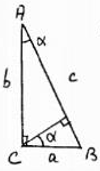
\includegraphics[width=0.12\textwidth]{lecture_07/pic1}
     	\end{center}
     \caption{triangle}
	\end{wrapfigure}

	\par $S_0 = c^2 f(\alpha)$
	\par $S_1 = b^2 f(\alpha)$
	\par $S_2 = a^2 f(\alpha)$
	\par $S = S_1 + S_2$
	\par $\Rightarrow c^2 = a^2 + b^2$

	\end{lecSection}
	
	\begin{lecSection}[Водородная связь	]
	\begin{figure}[H]
	Водородная связь является короткодействующим химическим взаимодействием.
	\begin{minipage}[h]{0.2\linewidth}
		\centering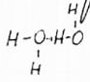
\includegraphics[width=\linewidth]{lecture_07/pic2}
		\caption{Водородная связь в воде ($3,6 \pm 0,5 \frac{\text{ккал}}{\textbf{моль}}$)}
	\end{minipage}
	\hfill
	\begin{minipage}[h]{0.2\linewidth}
		\centering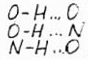
\includegraphics[width=\linewidth]{lecture_07/pic3}
		\caption{Сильная водородная связь}
	\end{minipage}
	\hfill
	\begin{minipage}[h]{0.2\linewidth}
		\centering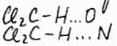
\includegraphics[width=\linewidth]{lecture_07/pic4}
		\caption{Слабая водородная связь}
	\end{minipage}
	\hfill
	\end{figure}
	
	\end{lecSection}
	
	\begin{lecSection}[Гидрофобное взаимодействие]
	\begin{flushleft}
	Характерно для маслоподобных вществ(например для парофинов). Две молекулы метана в воздухе(вакууме) имеют энергию взаимодействия(В-д-В) $2,5 \cdot 10^{-21}\text{Дж}$, а в воде $14\cdot 10^{-21}\text{Дж}$, то есть в воде притяжение сильнее.
	\par Изменение энергии Гиббса для 4-бутана в воде:
	\par $\Delta G = \Delta H - T\Delta S$
	\par $\Delta H = -4,3\frac{\text{кДж}}{\text{моль}}$; $T\Delta S = -28,7\frac{\text{кДж}}{\text{моль}} \Rightarrow \Delta G = +24,5 \frac{\text{кДж}}{\text{моль}}$ 
	\par Рвётся водородная сетка в воде $\rightarrow$ выталкивание, то есть это сводится к водородным связям.
	\par Общей теории гидрофобного взаимодействия нет.
	\end{flushleft}
	\end{lecSection}
	
	\begin{lecSection}[Мицеллы, образование мицеллы,микроэмульсии]
	\begin{flushleft}
		\begin{definition}
		Амфифильные вещества --- вещества, молекулы которых содержат и гидрофобные, и гидрофильные хвосты(Поверхностно-активные вещества(ПАВ) или детергенты)
		\end{definition}
	\par \textbf{ПАВы(детергенты):}
		\begin{itemize}
			\item Додецилсульфат натрия(SDS)
				\par $C_{12}H_{25}-OSO_3^--Na^+$
			\item Аэрозоль ОТ(АОТ)
				\begin{figure}[H]
				\begin{minipage}[h]{0.5\linewidth}
					\centering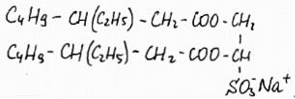
\includegraphics[width=\linewidth]{lecture_07/pic5}
				\end{minipage}
				\hfill
				\end{figure}
			\item Цетилтриметиламмония бромид — СТАВ(катионные детергенты)
				\par $C_{16}H_{33}-N^+(CH_3)-Br^-$
		\end{itemize}
		\par При определённых условиях ПАВы могут образовывать мицеллы $\Rightarrow$ можно растворять в воде гидрофобное вещество или же наоборот.
			\begin{figure}[H]
			\begin{minipage}[h]{0.7\linewidth}
				\centering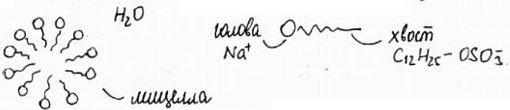
\includegraphics[width=\linewidth]{lecture_07/pic6}
			\end{minipage}
			\hfill
			\end{figure}
	
		\par Для большей устойчивости таких систем обычно добавляют спирт:
		\par ПАВ + вода + спирт = микроэмульсия($\Large \mu \varepsilon \normalsize$)
			\begin{figure}[H]
			\begin{minipage}[h]{0.2\linewidth}
				\centering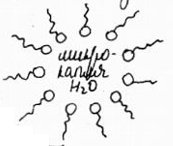
\includegraphics[width=\linewidth]{lecture_07/pic7}
				\caption{Обратная мицелла}
			\end{minipage}
			\hfill
			\begin{minipage}[h]{0.7\linewidth}
				\centering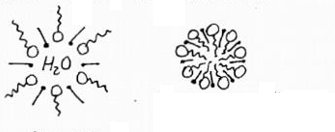
\includegraphics[width=\linewidth]{lecture_07/pic8}
				\caption{Микроэмульсия}
			\end{minipage}
			\hfill
			\end{figure}
		\par Хорошая микроэмульсия(АОТ + вода + изооктан) позволяет смоделировать мембрану.
		\par Типичные размеры таких конструкций $60-600\text{Å}$
		\par Радиус ядра: $R = (0,175\omega_0 + 1,5)\text{нм}$; $\omega_0 = \frac{[H_2O]}{\text{[АОТ]}}$
	\end{flushleft}
	\end{lecSection}

	\begin{lecSection}[Процесс мицеллообразования]
	
	\begin{wrapfigure}[5]{l}{0.2\textwidth}
    	\begin{center}
			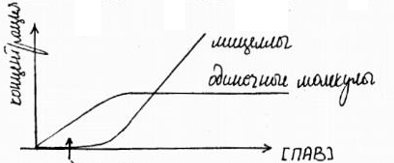
\includegraphics[width=0.6\textwidth]{lecture_07/pic9}
     	\end{center}
     \caption{Процесс мицеллообразования}
	\end{wrapfigure}
	\par $\uparrow$ --- критическая концентрация мицеллообразования
	\par В одном обычно 30 --- 60 молекул ПАВа
	\par Время пребывания детергента в мицелле $10^{-6} \text{c}$
	
	\end{lecSection}
		
\end{lecture}
